\documentclass[10pt,pdf,hyperref={unicode}]{beamer}

\mode<presentation>
{
\usetheme{boxes}
\beamertemplatenavigationsymbolsempty

\setbeamertemplate{footline}[page number]
\setbeamersize{text margin left=0.5em, text margin right=0.5em}
}

\usepackage[utf8]{inputenc}
\usepackage[english, russian]{babel}
\usepackage{bm}
\usepackage{multirow}
\usepackage{ragged2e}
\usepackage{indentfirst}
\usepackage{multicol}
\usepackage{subfig}
\usepackage{amsmath,amssymb}
\usepackage{enumerate}
\usepackage{mathtools}
\usepackage{comment}
\usepackage{multicol}
\usepackage{graphicx}
\usepackage{subcaption}
\usepackage[all]{xy}
\usepackage{bbm}

\usepackage{tikz}
\usetikzlibrary{positioning,arrows}

\tikzstyle{name} = [parameters]
\definecolor{name}{rgb}{0.5,0.5,0.5}

\usepackage{caption}
\captionsetup{skip=0pt,belowskip=0pt}
\renewcommand{\figurename}{}{}%  
\renewcommand{\figurename}{\relax}%

\makeatletter
\def\fnum@figure#1{\ignorespaces}
\makeatother

\newtheorem{rustheorem}{Теорема}
\newtheorem{russtatement}{Утверждение}
\newtheorem{rusdefinition}{Определение}

% colors
\definecolor{darkgreen}{rgb}{0.0, 0.2, 0.13}
\definecolor{darkcyan}{rgb}{0.0, 0.55, 0.55}

\AtBeginEnvironment{figure}{\setcounter{subfigure}{0}}

\captionsetup[subfloat]{labelformat=empty}

%----------------------------------------------------------------------------------------------------------

\title[Нейросетевые модели анализа выживаемости для решения задачи предсказания оттока абонентов]{Нейросетевые модели анализа выживаемости для решения задачи предсказания оттока абонентов}
\author{Е.\,В.\,Батарин}

\institute[]{Московский физико-технический институт}
\date[2022]{\small 27\;марта\;2025\,г.}

%---------------------------------------------------------------------------------------------------------
\begin{document}

\begin{frame}
\titlepage
\end{frame}

%----------------------------------------------------------------------------------------------------------
\section{Нейросетевые модели анализа выживаемости для решения задачи предсказания оттока абонентов}
\begin{frame}{Нейросетевые модели анализа выживаемости для решения задачи предсказания оттока абонентов}
\bigskip

\begin{block}{Задача}
Исследовать качество различных моделей предсказания оттока абонентов на основе методов анализа выживаемости
\end{block}
\begin{block}{Требуется}
Предложить метод, который: 
\justifying
\begin{enumerate}[1)]
\item Учитывает неполноту информации о факте оттока
\item Упорядочивает абонентов в зависимости от их времени оттока
\item Является интерпретируемым
\end{enumerate}
\end{block}
\begin{block}{Решение}
Использовать нейросетевую модель с дискретным временем со специально подобранной функцией потерь
\end{block}
\end{frame}

%---------------------------------------------------------------------------------------------------------
\section{Обозначения}
\begin{frame}{Обозначения}


$\mathcal{T}=\{0,\ldots,T_{\max}\}$ - дискретное время

$\mathcal{K}=\{\emptyset,1\}$ - множество событий: цензурирование и отток

$\tau^i=\min(T^i,C^i) \in\mathcal{T} $ - право-цензурированные отсчеты времени

$\mathcal{X}^i(t)=\{\mathbf{x}^i(t_j^i):0\leq t_j^i\leq t\mathrm{~for~}j=1,\cdots,J^i\}$ - вектора признаков 

$\mathcal{D}=\{(\mathcal{X}^i,\tau^{i},k^{i})\}_{i=1}^{N}$ - обучающая выборка



{\fontsize{8.5}{10}\selectfont
	\begin{align*}
		& \begin{aligned}
			F_{k^{*}}(\tau^{*}|\mathcal{X}^{*}) & = P(T\leq\tau^{*},k=k^{*}|\mathcal{X}^{*},T>t_{J^{*}}^{*}) \\
			& =\sum_{\tau\leq\tau^*}P(T=\tau,k=k^*|\mathcal{X}^*,T>t_{J^*}^*).
		\end{aligned}
		\quad
		& \begin{aligned}
			S(\tau^{*}|\mathcal{X}^{*}) & = P(T>\tau^*|\mathcal{X}^{*},T>t_{J^*}^{*}) \\
			& =1-\sum_{k\neq\emptyset}F_k(\tau^*|\mathcal{X}^{*}).
		\end{aligned} \\
		% Подписи под формулами без смещения формул
		& \text{Функция распределения для события $k^*$}
		& \hspace{55pt} \text{Функция выживания}
	\end{align*}
}



\end{frame}


%---------------------------------------------------------------------------------------------------------
\section{Иллюстрация правого цензурирования}
\begin{frame}{Иллюстрация правого цензурирования}



\begin{figure}[h!]
	\centering
	\begin{minipage}{1\textwidth}
		\centering
		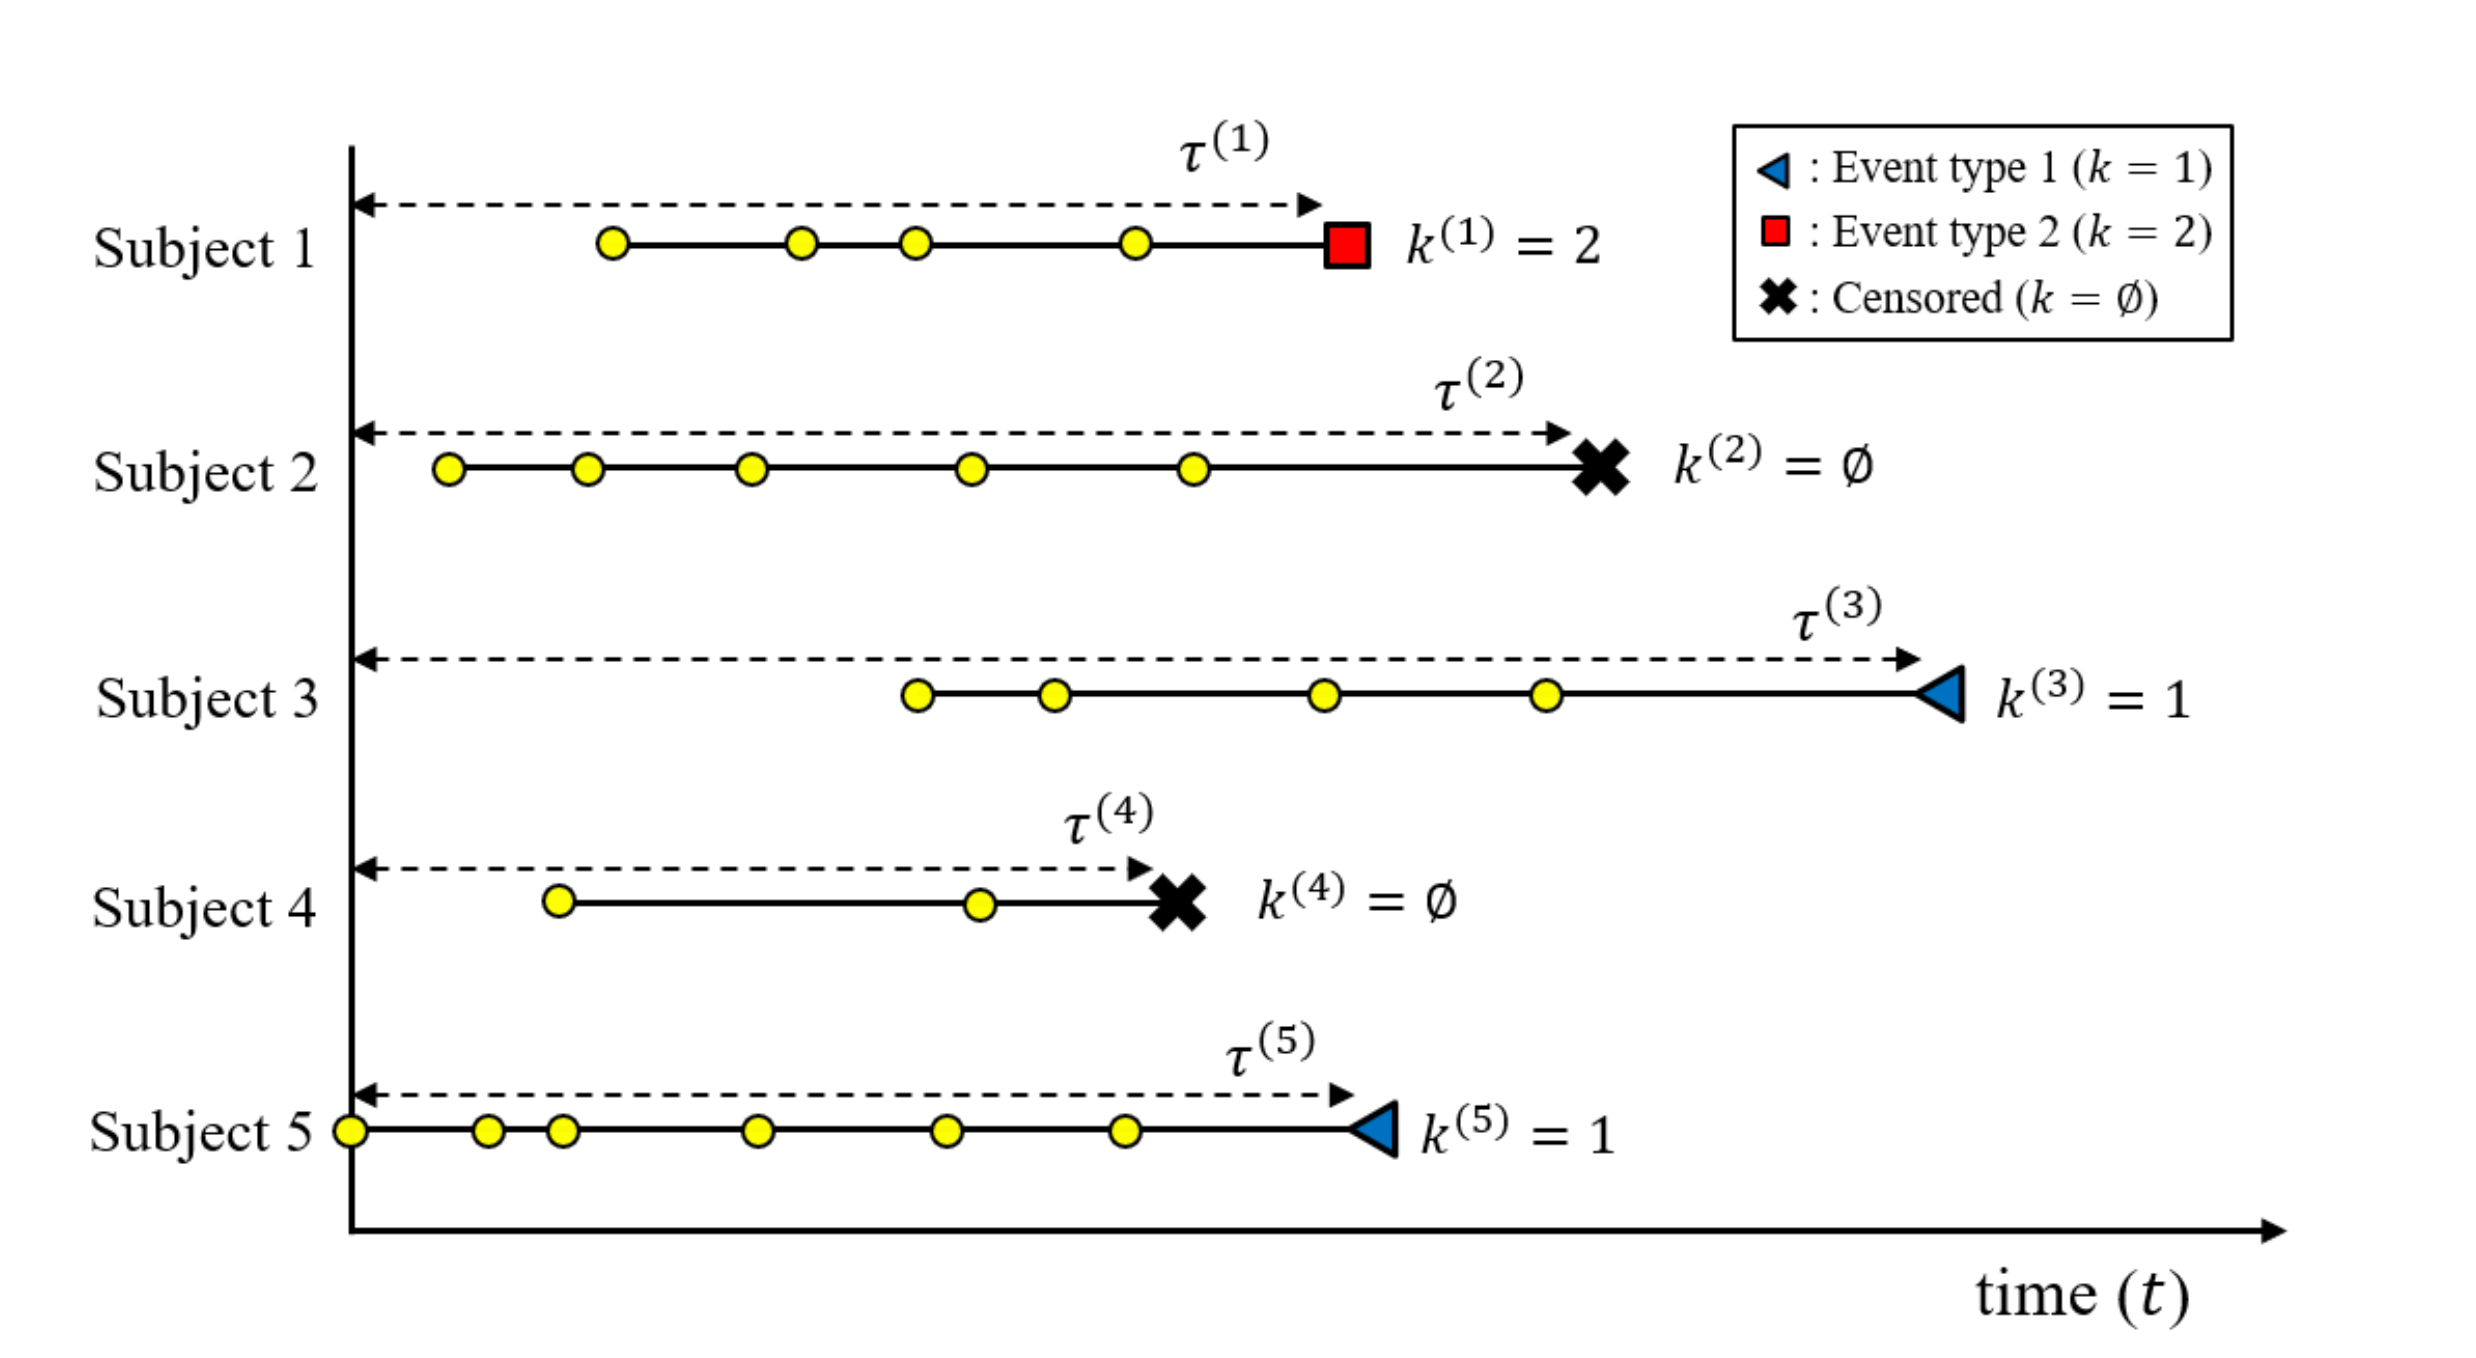
\includegraphics[width=0.9\linewidth]{../figures/survival_example.png}
		\renewcommand{\figurename}{}{}%
		\caption{Цензурирование абонентов}
	\end{minipage}

\end{figure}

\end{frame}
%----------------------------------------------------------------------------------------------------------

\section{Предложенный метод}
\begin{frame}{Предложенный метод}
	
	\begin{block}{Постановка задачи}
		На основе обучающей выборки $\mathcal{D}$ построить аппроксимации функции распределения и функции выживаемости: $\hat{F}_{k^*}(\tau^*|\mathcal{X}^*)$ и $\hat{S}(\tau^{*}|\mathcal{X}^{*}) =1-\sum_{k\neq\emptyset}\hat{F}_{k^*}(\tau^*|\mathcal{X}^{*})$
	\end{block}
	
	\begin{block}{Функция потерь}
		Задача сводится к минимизации функции $\mathcal{L}_{\mathrm{Total}}=\mathcal{L}_1+\mathcal{L}_2+\mathcal{L}_3$, которая состоит из слагаемых:
		
		\scriptsize
		\[
		\begin{aligned}
			\mathcal{L}_{1} = -\sum_{i=1}^N \biggl[ 
			&\mathbbm{1}(k^i\neq\emptyset)\cdot\log\left(
			\frac{o_{k^i,\tau^i}^i}{
				1-\sum_{k\neq\emptyset}\sum_{n\leq t_{Ji}^i}o_{k,n}^i}
			\right) 
			 +\mathbbm{1}(k^i=\emptyset)\cdot\log\left(
			1-\sum_{k\neq\emptyset}\hat{F}_k(\tau^i|\mathcal{X}^i)
			\right)
			\biggr]
		\end{aligned}
		\]
		
		
		\scriptsize
		\[
		\begin{aligned}
		\mathcal{L}_2=\sum_{k=1}^K\alpha_k\sum_{i\neq j}A_{kij}\cdot\eta\left(\hat{F}_k(s^i+t_{J^i}^i|\mathcal{X}^i),\hat{F}_k(s^i+t_{J^j}^j|\mathcal{X}^j)\right)
		\end{aligned}
		\]
		
		\scriptsize
		\[
		\begin{aligned}
		\mathcal{L}_3=\beta\cdot\sum_{i=1}^N\sum_{j=0}^{J^i-1}\sum_{d\in\mathcal{I}}(1-m_{j+1,d}^i)\cdot\zeta(x_{j+1,d}^i,y_{j,d}^i)	
		\end{aligned}
		\]
		где $s^i=\tau^i-t_{J^i}^i$, $A_{kij}=\mathbbm{1}(k^i=k,s^i<s^j)$ , $\eta(a,b)=\exp\left(-\frac{a-b}{\sigma}\right)$, $o_{k,n}^i$ - выходы модели

	\end{block}
	

	
	
\end{frame}
%----------------------------------------------------------------------------------------------------------





\section{Архитектура модели}
\begin{frame}{Архитектура модели }
	
	
	\begin{figure}[h!]
		
		\begin{minipage}{0.8\textwidth}
			\centering
			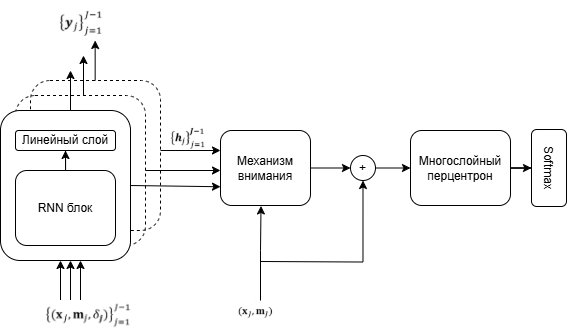
\includegraphics[width=\linewidth]{../figures/dynamic_deephit_scheme_only_architecture.png}
			\renewcommand{\figurename}{}{}%
		\end{minipage}
	\end{figure}
	
	
\end{frame}

%----------------------------------------------------------------------------------------------------------
\section{Критерии качества модели анализа выживаемости}
\begin{frame}{Критерии качества модели анализа выживаемости}

\begin{block}{Определение $C$-индекса}

Пусть для пары абонентов $(i,j)$ определены $\tau_i$  < $\tau_j$ - моменты времени (возможно, цензурированные), $\delta_i$ - индекс цензурирования, равный $0$, если $\tau_i$ право-цензурировано и $1$ - в противном случае. Также обозначим через $\hat{F}_{k,i}$ и $\hat{F}_{k,j}$ вероятности оттока до момента по событию $k$ времени $\tau_i$ для абонентов $i$ и $j$ соответственно (оцененные моделью функции распределения). Тогда C-индекс определяется следующим образом:

$$C\text{-}index =
\frac{
	\sum\limits_{i,j} \mathbf{1}_{\tau_i < \tau_j} \cdot \mathbf{1}_{\hat{F}_{k,i} > \hat{F}_{k,j}} \cdot \delta_i
}{
	\sum\limits_{i,j} \mathbf{1}_{\tau_i < \tau_j} \cdot \delta_i
}$$	
	
	
\end{block}


\begin{block}{Понятие верно упорядоченной пары}

Пара абонентов $(i,j)$ считается верно упорядоченной (отранжированной), если для оцененных моделью функций распределений $\hat{F}_{k,i}$ и $\hat{F}_{k,j}$ выполнено неравенство: 

$$ \hat{F}_{k,i}(\tau_i ) >  \hat{F}_{k,j}(\tau_i ) $$ 

	
\end{block}
	
\end{frame}

%----------------------------------------------------------------------------------------------------------
\section{Свойство добавки $\mathcal{L}_2$}
\begin{frame}{Свойство добавки $\mathcal{L}_2$}
	
\begin{block}{Определение отступов}
	
		Пусть $(i,j)$ - пара абонентов, для которых произошло событие оттока $k$ в моменты времени $\tau^{(i)}$ и $\tau^{(j)}$ соответственно, причем $\tau^{(i)} < \tau^{(j)}$. Тогда $M_{k,i,j}$ определяется как
		
		$$M_{k,i,j} = \hat{F}_k(s^i+t_{J^i}^i|\mathcal{X}^i) - \hat{F}_k(s^i+t_{J^j}^j|\mathcal{X}^j)$$
		
\end{block}


\begin{block}{Основное свойство}
	Пусть $$\mathcal{L}_2 =\sum_{k=1}^K\alpha_k\cdot\sum_{i\neq j}A_{k,i,j}\cdot\eta\left(\hat{F}_k(s^i+t_{J^i}^i|\mathcal{X}^i) , \hat{F}_k(s^i+t_{J^j}^j|\mathcal{X}^j))\right)$$ добавка к функции потерь. Тогда $\mathcal{L}_2$ является убывающей от отступов функцией.  
\end{block}

\end{frame}
%----------------------------------------------------------------------------------------------------------
\section{Описание вычислительного эксперимента}
\begin{frame}{Описание вычислительного эксперимента}
	
	\begin{block}{Цель эксперимента}
	\begin{enumerate}[1)]
	\item Проследить влияние новых признаков - выходов предложенной модели - на точность решения задачи классификации абонентов
	\item Оценить значимость новых признаков
\end{enumerate}		
		
		
	\end{block}
	
	
	\begin{block}{Описание датасета}
	\begin{enumerate}[1)]
		\item Базовый сегмент: обучение - B2C абоненты Мегафона в июне и июле 2024, тест - в августе 2024. Обучающая выборка содержит 12 миллионов примеров и сбалансирована. Тестовая выборка содержит 3 миллиона примеров и не сбалансирована
		\item Целевое событие: 4 класса - отток в конце 1, 2 и 3 месяц и отсутствие оттока
		\item Исходные признаки: 50 признаков абоненской активности
	\end{enumerate}
	\end{block}
	
		\begin{block}{Выходной вектор модели}
	Новые признаки, генерируемые моделью, представляют собой вектор $(x_0,x_1,x_2,x_3,x_4) \in \mathbb{R}^{5}$, где $x_i$ - вероятность выживания в $i$-ый месяц, где за $0$ месяц берется июнь 2024
	\end{block}
	
\end{frame}


%----------------------------------------------------------------------------------------------------------
\section{Результаты вычислительных экспериментов}
\begin{frame}{Результаты вычислительных экспериментов}
	
	\begin{block}{Точность предсказания}
		\begin{enumerate}[1)]
		\item Только новые признаки: $75.5\%$
		\item Только исходные признаки: $80.6\%$
	\end{enumerate}	

		
	\end{block}
	
	
	\begin{block}{Значимость признаков}
 
 	\begin{figure}[h!]
 	
 	\begin{minipage}{0.8\textwidth}
 		\centering
 		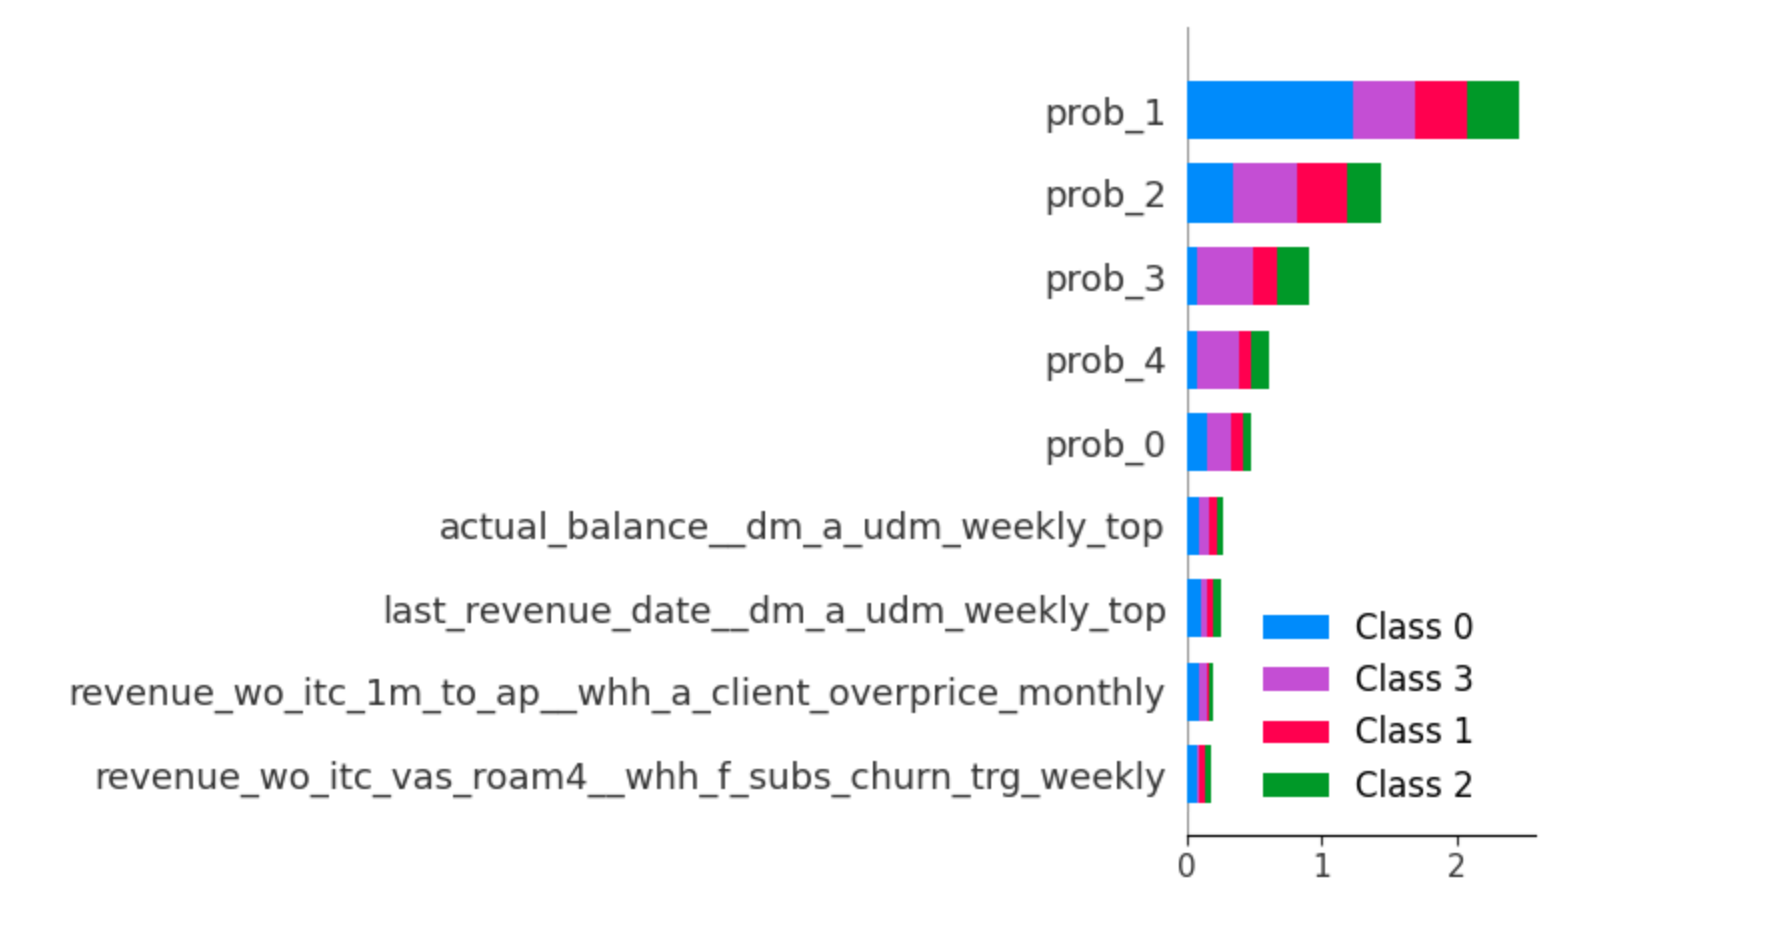
\includegraphics[width=\linewidth]{../figures/deephit_shap_baseline1.2.png}
 		\renewcommand{\figurename}{}{}%
 	\end{minipage}
 \end{figure}
 
	\end{block}
	
\end{frame}



%----------------------------------------------------------------------------------------------------------
\section{Посылки на защиту}
\begin{frame}{Выводы}
	\justifying
	\begin{minipage}{0.85\textwidth} % уменьшаем ширину области до 85% от слайда
		\begin{enumerate}
			\justifying
			\item Предложена нейросетевая модель анализа выживаемости с дискретным временем для решения задачи предсказания оттока абонентов 
			
			\item Построена специфическая для задачи функция потерь и обосновано свойство ее добавки $\mathcal{L}_2$
			
			\item Проведен вычислительный эксперимент, в котором показано, что применение модели анализа выживаемости позволяет получить новые признаки, которые: 
			\begin{itemize}
				\item Имеют наибольшую SHAP-значимость
				\item Вносят вклад в точность предсказаний, сопоставимый с исходными признаками
			\end{itemize}
		\end{enumerate}
	\end{minipage}
\end{frame}

%----------------------------------------------------------------------------------------------------------

\end{document} 